% !TeX spellcheck = de_CH
%%%%%%%%%%%%%%%%%%%%%%%%%%%%%%%%%%%%%%%%%%%%%%%%%%%%%%%%%%%%%%%%%
%  _____   ____  _____                                          %
% |_   _| /  __||  __ \    Institute of Computitional Physics   %
%   | |  |  /   | |__) |   Zuercher Hochschule Winterthur       %
%   | |  | (    |  ___/    (University of Applied Sciences)     %
%  _| |_ |  \__ | |        8401 Winterthur, Switzerland         %
% |_____| \____||_|                                             %
%%%%%%%%%%%%%%%%%%%%%%%%%%%%%%%%%%%%%%%%%%%%%%%%%%%%%%%%%%%%%%%%%
%
% Project     : BA Welti Keller
% Title       : 
% File        : resultate.tex Rev. 00
% Date        : 15.09.2014
% Author      : Tobias Welti
%
%%%%%%%%%%%%%%%%%%%%%%%%%%%%%%%%%%%%%%%%%%%%%%%%%%%%%%%%%%%%%%%%%

\chapter{Resultate}\label{chap.resultate}

\section{Testfälle}
Die wichtigsten Testfälle für die grundsätzliche Funktionalität der Messstation konnten erfolgreich abgeschlossen werden. Für einige Tests blieb jedoch nicht genügend Zeit vor der Fertigstellung des Berichts. Diese Tests werden so weit möglich noch nachgeholt.

Im Kapitel \ref{chap.tests} ab Seite \pageref{chap.tests} sind die Testfälle und die Testergebnisse aufgeführt.


Zum Zeitpunkt des Verfassens dieses Berichts konnten keine weiteren Tests durchgeführt werden. Geplant währen

\section{Ereigniserkennung}
Der \gls{adwandler} des \emph{NXP LPC4088} \gls{mc} wurde wie geplant in Betrieb genommen und liefert Messdaten, die sich sehr gut mit dem analogen Ausgangssignal des \gls{sensor}s decken. Abbildung \ref{fig.comparison} zeigt den Vergleich zwischen der Messung von Oszilloskop (blau) und der \gls{sensoreinh} (grün). Die \gls{sensoreinh} arbeitete mit einer \gls{fs} von 10000~\ensuremath{Hz}, das Oszilloskop zeichnete mit einer \gls{fs} von 3.125~MHz auf. Um ein Ereignis zu simulieren, wurde ein Golfball auf den Testaufbau (siehe im Verzeichnis Fotos/Testaufbau/ auf der beiliegenden CD) fallen gelassen. Der Vergleich zeigt, dass die beiden Kurven gut übereinstimmen. 

\begin{figure}
	\centering
		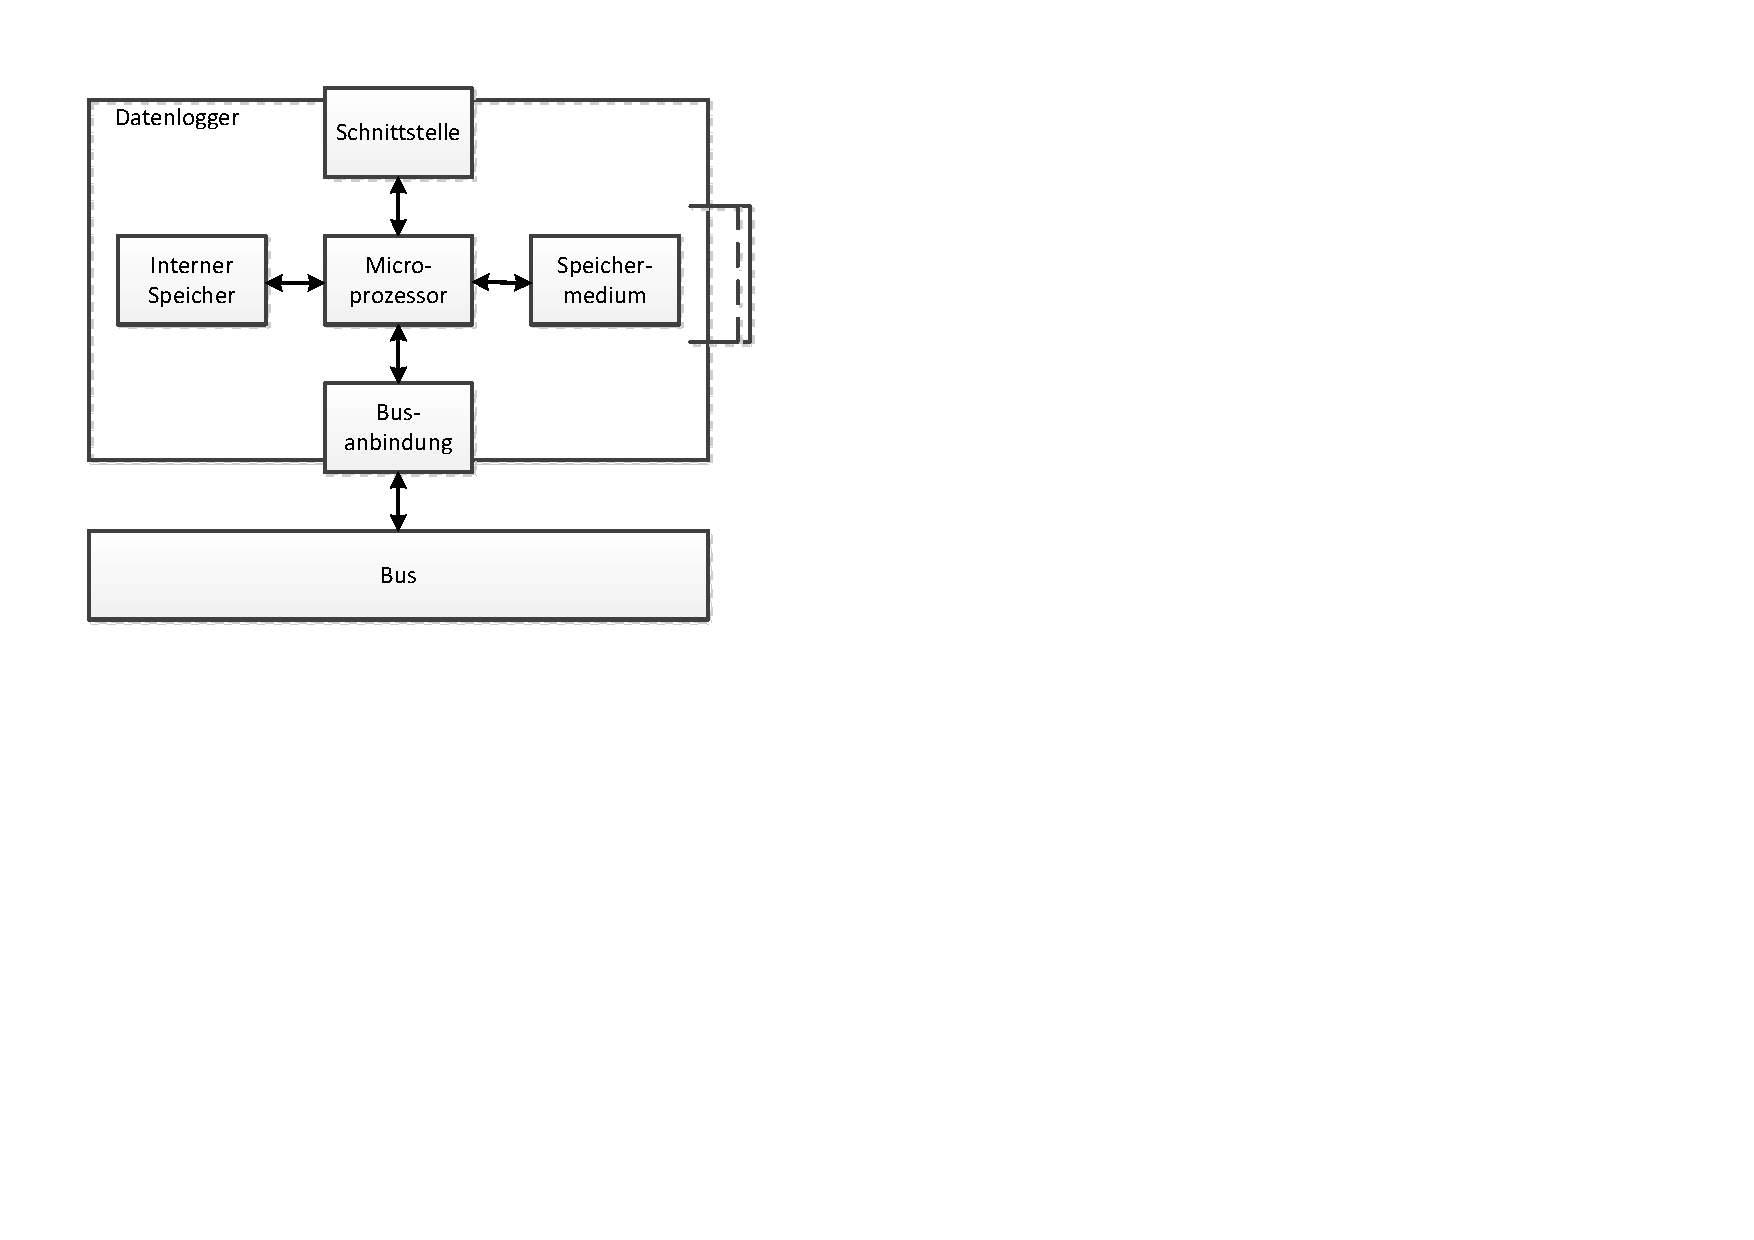
\includegraphics[width=0.8\textwidth]{images/visio/hardwarekonzept_logger.pdf}
	\caption{Vergleichsmessung mit Oszilloskop und \gls{sensoreinh}.}
	\label{fig.comparison}
\end{figure}


Der Betrieb mit 10000~Hz war für unseren Testaufbau genügend, die Peaks traten mit einer Frequenz von ungefähr 2000~Hz auf. Die Frequenz der Peakspitzen variiert sowohl mit der Plattenkonstruktion als auch mit der Korngrösse, Kornbeschaffenheit und der Art des Aufschlags. Daher muss für den tatsächlichen Messbetrieb eine Kalibrierung gemacht werden, um die geeigneten Parameter zu finden.

Für Versuche mit verschiedenen \gls{fs} blieb keine Zeit mehr. So können wir zur Zeit nicht sagen, was die höchstmögliche \gls{fs} mit der aktuellen Software ist.

\section{Daten-Reduktion und -Speicherung}
Die Datenreduktion durch Wahl der verschiedenen Detail-Level ist effizient gelöst und sehr effektiv. Pro Messwert müssen lediglich zwei Vergleiche für die Bestimmung des Signalpegels gemacht werden, sowie zwei Vergleiche mit je einem vorhergehenden Wert für die Bestimmung des Peak-Maximums und des Ereignis-Maximums.

Die Wahl des Detail-Levels beeinflusst lediglich, welche Daten übertragen werden. Auf die Zwischenspeicherung hat sie keinen Einfluss. Vor und nach der Übertragung finden keine komplexen Umrechnungen an den Messdaten statt. Die \gls{bitbreite} wird von 12 Bit auf 8 Bit reduziert. Die grösste Datenreduktion erfolgt durch die Auswahl der relevanten Daten.

\subsection{Rohdaten (raw)}
Es werden alle Messpunkte übertragen und gespeichert. Es findet keine Datenreduktion statt. Pro Messpunkt fällt 1 Byte an. Bei einer \gls{fs} von 10000~Hz resultiert ein Datenstrom von 10000~Byte/s.

\subsection{Detaillierte Ereignisdaten (detailed)}
Es werden nur die Messpunkte der Ereignisse gespeichert. Messpunkte, die nicht zu einem Ereignis gehören, werden verworfen. Der Datenstrom variiert daher mit der Häufigkeit der Ereignisse. Liegt zu 10 \% der Messzeit ein Ereignis vor, wird dies von der \gls{wsl} als hohes Geschiebeaufkommen eingestuft. Eine solche Periode kann über mehrere Stunden anhalten, ist aber nicht jeden Tag zu erwarten.

Bei 10 \% Ereigniszeit wird in diesem Modus eine Datenreduktion um 90 \% erzielt. Für die durchschnittliche Ereigniszeit nehmen wir 5 \% an. Dann resultiert pro \gls{sensor} ein Datenstrom von 500~Byte/s.

\subsection{Peaks (peaks only)}
Der Timestamp, die Dauer des Ereignisses, die Anzahl \glspl{peak} und alle Peakspitzen werden gespeichert. Pro Ereignis fallen 8 Byte an für die Eckdaten und 2 Byte pro Peak. Ein Ereignis hat im Normalfall weniger als 20 Peaks. Wir nehmen somit 48 Byte pro Ereignis an. Bei einem Ereignis pro Sekunde resultiert ein Datenstrom von rund 50 Byte/s.

\subsection{Minimale Daten (sparse)}
Es werden nur der Timestamp, die Dauer des Ereignisses, die Anzahl \glspl{peak} und der maximale Ausschlag des Ereignisses übertragen, das sind 8 Byte pro Ereignis. Der Datenstrom erreicht so lediglich 8 Byte/s.

\subsection{Messdauer}
Je nach Modus fallen sehr unterschiedliche Datenströme pro Sensor an. Ein Vergleich, wie lange mit einem GByte Speicherplatz gemessen werden kann, ist in Tabelle \ref{table.datarate} aufgeführt. Anhand dieser Werte kann abgeschätzt werden, wie lange eine Messstation ohne Wechsel des Speichermediums betrieben werden kann.

\begin{table}
\begin{tabular}{|l|l|l|}
\hline \textbf{Detail-Level} & \textbf{Byte/s} & Messzeit/GByte\\ 
\hline raw                   & 10000 & 27~h \\
\hline detailed              &   500 & 23~d \\
\hline peaks only            &    50 & 231~d \\
\hline sparse                &     8 & 3.9~yr \\
\hline 
\end{tabular}
\caption{Vergleich des Datenaufkommens verschiedener Detail-Levels.}
\label{table.datarate}
\end{table} 

\section{Hardware}
Für den Datenlogger und die Sensoreinheiten wurde mit der Hilfe von Erich Ruff (ZHAW InES) und Valentin Schlatter (ZHAW InES) eine Leiterplatte entworfen sowie Gehäuse gebaut. Die Leiterplatte wurde so entworfen, dass über die Bestückung entschieden wird, ob ein Datenlogger oder eine Sensoreinheit gebaut wird. Für einen Datenlogger wird die Leiterplatte mit einem SD-Karten-Slot bestückt. Für die Sensoreinheit wird ein Tiefpassfilter und der Anschluss für den Sensor bestückt. Beide Varianten enthalten die Spannungsversorgung (12~V auf 5~V), einen CAN-Transceiver und die Anschlüsse für die Kabel. Der Schaltplan und das Leiterplattenlayout befinden sich im Anhang \ref{app.pcb}